% LuaLaTeX document — compile with:
%   cd docs && lualatex shear_lattice_renormalisation.tex   (run twice)
\documentclass[11pt,a4paper]{article}

\usepackage{fontspec}
\setmainfont{Latin Modern Roman}
\setmonofont{Latin Modern Mono}

\usepackage{amsmath,amssymb,bm}
\usepackage{booktabs}
\usepackage{geometry}
\geometry{margin=2.5cm}
\usepackage{hyperref}
\hypersetup{colorlinks=true,linkcolor=blue!60!black,urlcolor=blue!70!black}
\usepackage{enumitem}
\usepackage{xcolor}
\usepackage{pgfplots}
\pgfplotsset{compat=1.18}
\usepackage{tcolorbox}

\newcommand{\Dmu}{\Delta\mu}
\newcommand{\Dlam}{\Delta\lambda}
\newcommand{\Drho}{\Delta\rho}
\newcommand{\Kren}{K}

\title{A lattice renormalisation of the shear depolarisation\\
of a cubic voxel\\[6pt]
\large Identification, measurement, and correction of the residual error\\
in a space-filling cubic-voxel discretisation}
\author{Tod Nestor}
\date{September 2026}

\begin{document}
\maketitle

\begin{abstract}
A uniform elastic slab discretised into a space-filling lattice of identical
cubic voxels, each carrying the analytic single-site cube T-matrix and coupled by
an exact Foldy--Lax solve, does not reproduce the homogeneous layer it is made
of. A relative error of $8.6\times10^{-4}$ survives refinement: halving the cell
size does not reduce it. We report the identification of that residual and its
removal.

The residual is shown to be (i) static, (ii) quadratic in contrast, (iii)
independent of the supercell size, and (iv) confined \emph{entirely} to the shear
channel --- the dilatational and density channels converge cleanly to zero. It is
then shown to be a single wrong scalar: the effective shear contrast carried by a
voxel. Correcting that scalar reduces the discrepancy against the exact
reflectivity solution from $2.9\times10^{-3}$ to $\sim\!10^{-8}$.

The correction is a constant factor on the cube's \emph{depolarisation},
\[
  \Kren \;=\; \frac{1-A^{\text{eff}}_{\varepsilon,\text{diag}}}
                   {1-A^{\text{iso}}_{\varepsilon,\text{diag}}}
        \;=\; 0.8862 ,
\]
constant to $0.3\%$ over a sixteen-fold range of contrast, flat in frequency
until $ka$ grows, and \emph{predictive}: extracted from pure positive shear
alone, it transfers to mixed contrasts and to negative shear, and leaves
untouched the two channels that require no correction. With it applied the
scheme converges under refinement instead of saturating.

The constant is measured, universal and predictive. \textbf{It is not derived},
and this document says so throughout. $8/9$ is excluded.
\end{abstract}

\tableofcontents

%======================================================================
\section{The problem}
%======================================================================

\subsection{An identity that the discretisation must satisfy}

Take a homogeneous elastic slab of thickness $H$ whose properties differ from the
background by $(\Dlam,\Dmu,\Drho)$, and represent it as an $M\times M\times N_z$
lattice of identical cubes of side $d$, space-filling, with $N_z d = H$. Each cube
carries the analytic Rayleigh cube T-matrix; the cubes are coupled by the
Foldy--Lax system $(\bm{I}-\bm{G}_0\bm{T}_0)\psi=\psi^0$.

The medium so constructed \emph{is} the homogeneous slab. Every cube is identical
and they tile space without gaps, so the exact plane-wave reflection coefficient
is the one the Kennett reflectivity recursion returns in closed form. Agreement
is therefore an \textbf{identity}, not a modelling approximation, and any
disagreement is a defect of the discretisation.

Two further identities follow and are used throughout as controls:
\begin{enumerate}[nosep]
  \item the answer cannot depend on $M$, the number of identical cubes called one
    repeating unit;
  \item the answer must converge as $d\to0$ at fixed $H$.
\end{enumerate}

\subsection{What was observed}

Neither held. Refining the voxelisation at fixed physical thickness made the
answer \emph{worse}, and the error grew without sign of settling:

\begin{center}
\begin{tabular}{rrr}
\toprule
$n_z$ & $d$ (m) & relative error \\
\midrule
 1 & 4.000 & $3.95\times10^{-3}$ \\
 2 & 2.000 & $8.29\times10^{-3}$ \\
 4 & 1.000 & $1.37\times10^{-2}$ \\
 8 & 0.500 & $2.03\times10^{-2}$ \\
16 & 0.250 & $2.62\times10^{-2}$ \\
\bottomrule
\end{tabular}
\end{center}

Refinement is the only instrument a discretisation has for buying accuracy, and
here it bought error.

%======================================================================
\section{Two defects had to be removed before the residual was visible}
%======================================================================

The growth above turned out to be two separate faults stacked on a third. They
are reported first because every measurement in this document depends on their
removal, and because the original diagnosis of the residual was taken in their
presence and was wrong as a result.

\subsection{The periodic lateral sum was truncated}

The periodic kernel assembled the horizontal propagator only over
$\Delta x,\Delta y\in[-(M{-}1),M{-}1]$ --- a single $(2M-1)^2$ patch --- and then
wrapped it for the circular convolution. That is not a lattice sum. It was caught
not by a convergence expectation but by identity~(1) above: a laterally uniform
layer cannot depend on $M$, and it did, obeying
$\text{error}=1.12\times10^{-3}+1.15\times10^{-2}/M$.

The repair is an exact Bloch sum written directly at the $M^2$ discrete Bloch
points, by Ewald summation at equal depth and by reciprocal summation of the
spectral kernel between depth planes. After it, $M=2,3,4,6,8$ agree to
$5.05\times10^{-13}$ --- the identity holds.

\begin{tcolorbox}[colback=yellow!6,colframe=yellow!45!black,title=Consequence for earlier results]
At $M=4$, used throughout the earlier campaign, \textbf{63\%} of the reported
``discretisation floor'' was this artifact, and because it accumulated plane by
plane it produced most of the \emph{growth} as well. Results taken before the
repair required re-running, not reinterpretation.
\end{tcolorbox}

\subsection{The contact propagator was a midpoint rule}

The inter-cell operator should be the doubly volume-averaged (Galerkin) object
$\langle\langle \bm{G}\rangle\rangle$; collocating at cell centres is a midpoint
rule whose error at \emph{contact} does not fall with refinement, because
(cell size)/(separation) is unity at every scale. Measured against the analytic
$O_h$ tables, the point value is wrong by $130\%$ at face contact, $42\%$ at
edge, $9.3\%$ at corner.

\subsection{What remained}

With the lateral sum exact and the Galerkin contact correction applied, the
ladder flattens:

\begin{center}
\begin{tabular}{rrrr}
\toprule
$n_z$ & truncated & exact sum & exact $+$ Galerkin contact \\
\midrule
1 & $3.95\times10^{-3}$ & $1.47\times10^{-3}$ & $7.73\times10^{-4}$ \\
2 & $8.29\times10^{-3}$ & $3.36\times10^{-3}$ & $8.35\times10^{-4}$ \\
4 & $1.37\times10^{-2}$ & $4.33\times10^{-3}$ & $8.51\times10^{-4}$ \\
8 & $2.03\times10^{-2}$ & $4.81\times10^{-3}$ & $8.58\times10^{-4}$ \\
\bottomrule
\end{tabular}
\end{center}

The scheme now converges --- but to $8.6\times10^{-4}$, not to zero. That
residual is the subject of the rest of this document.

%======================================================================
\section{Experimental procedure: elimination}
%======================================================================

Each suspect was tested by a measurement with a pre-stated outcome, and every one
of the first four was refuted. They are recorded because the refutations
constrain the answer as much as the confirmation does, and because three of them
are natural enough to be proposed again.

\subsection{Signature of the residual}

Established first, since it is what the suspects must match:
\begin{description}[style=nextline,leftmargin=1.2em]
  \item[Saturating] error ratio $\to1.00$ across $n_z=1\ldots32$; it is a
    per-cell error that refinement cannot dilute.
  \item[Independent of $M$] to six digits, so it is physical and not a residue of
    the lattice sum.
  \item[Static] the log--log slope in $\omega$ is $-0.02$.
  \item[Quadratic in contrast] absolute error $\propto c^{1.98}$ over the range
    where the measurement stands above the numerical floor of the pipeline. This
    matters: a \emph{quadrature} error is linear in the contrast, and the
    truncation artifact of \S2.1 measured $c^{1.00}$ exactly.
\end{description}

\begin{tcolorbox}[colback=gray!5,colframe=black!62,
  title={A measurement discipline used throughout}]
Below $c\approx10^{-2}$ the absolute discrepancy falls to $10^{-12}$ and under,
which is the numerical floor of the solve. Those points were \emph{excluded} from
the fit rather than fitted through: including them drags the exponent from $1.98$
to $1.80$. The same rule --- show an arbiter converged before letting it convict
anything --- is applied to every direct lattice sum in this work.
\end{tcolorbox}

\subsection{Refuted: the averaged propagator's dynamic truncation}

The volume-averaged operator retains dynamic corrections to $\mathcal{O}(\omega^4)$
and so carries an $\mathcal{O}(\omega^6)$ error, relatively $\mathcal{O}((kd)^2)$.
Refining eight-fold should then reduce it sixty-four-fold.

\emph{Measured:} static, $+\omega^2$ and $+\omega^4$ tables agree to
$5.7\times10^{-3}$ relative --- the \textbf{static} table alone reproduces the
answer --- and the residual does not move with $d$. Refuted twice over.

\subsection{Refuted: the isolated-cube depolarisation as a whole}

The cube T-matrix carries amplification factors $A$ built from $\Gamma_0$, the
self-interaction of a cube in an infinite \emph{host}. In a space-filling tiling
a cube's neighbours are not host material, so one may suspect the depolarisation
is a correction the lattice has already cancelled.

\emph{Measured:} setting $A=1$ makes the answer $\mathbf{24.6\times}$
\textbf{worse} ($8.5\times10^{-4}\to2.09\times10^{-2}$), at every rung and every
contrast. The depolarisation is most of the physics and it stays. The partition
--- $\Gamma_0$ the voxel's own self-field, $\bm{G}_0$ carrying every other voxel
--- is correct.

\begin{tcolorbox}[colback=red!4,colframe=red!45!black,title=A refutation that was later shown to be too coarse]
This result was initially read as closing the lattice-renormalisation question.
It does not. $A=1$ removes \emph{one hundred percent} of the depolarisation,
whereas the correction established in \S4 is \emph{one third of one percent}. The
test was three orders of magnitude too blunt to detect what was there. A null
result from a coarse instrument is not evidence of absence.
\end{tcolorbox}

\subsection{Refuted: the 27-component single-site response}

The nine-component basis represents the exciting field by value and gradient at
the cell centre; the quadratic modes of the 27-component Galerkin T-matrix
represent its curvature.

\emph{Measured:} substituting the $T_{27}$ strain sector makes the answer
$3\times$ \emph{worse} ($8.61\times10^{-4}\to2.61\times10^{-3}$).

This is \textbf{not} a refutation of $T_{27}$. It is a refutation of the
\emph{pairing}: a 27-mode single-site response was driven through a nine-mode
propagator. The companion derivation of the generalised inter-voxel propagator
states in advance that for $T_{27}$ ``the propagator must couple all 27 modes''.
The measurement confirms that warning rather than testing the physics.

\subsection{Refuted: propagator averaging beyond contact}

\emph{Measured:} extending the double average beyond the contact shell makes the
answer $32\%$ worse ($8.51\times10^{-4}\to1.12\times10^{-3}$), converged in the
quadrature order. Sensitivity analysis shows why this is not simply a bug: all
Chebyshev shells influence the answer comparably ($\mathrm{d}(\text{err})/
\mathrm{d}\epsilon \approx -1.7,+1.8,+1.8\times10^{-3}$ for shells $1,2,3$), so
the residual is not localised at contact, and reproducing it would require an
implausible $\sim\!50\%$ error in some shell's coupling.

%======================================================================
\section{Identification: the residual is one scalar in the shear channel}
%======================================================================

\subsection{Splitting by channel}

Running each contrast channel alone is decisive:

\begin{center}
\begin{tabular}{lrrl}
\toprule
case & $A_\theta$ & residual & behaviour under refinement \\
\midrule
pure density & $1.000000$ & $1.41\times10^{-5}$ & converges, ratios $0.247/0.249/0.249$ \\
pure $\lambda$ & $0.968992$ & $1.19\times10^{-5}$ & converges \\
pure $\mu$ & $0.989446$ & $2.89\times10^{-3}$ & saturates \\
working (all three) & $0.959079$ & $8.51\times10^{-4}$ & saturates \\
\bottomrule
\end{tabular}
\end{center}

Two conclusions. First, the density and dilatational channels are \emph{already
correct}: they converge at clean second order towards zero. Second, the residual
is \textbf{anti-correlated} with the amplification $A_\theta$ --- pure $\lambda$
carries more depolarisation and $240\times$ less residual --- which independently
exonerates the amplification factors as such and locates everything in the shear
channel.

\subsection{Scanning the effective shear contrast}

At normal incidence a P wave excites only normal strains, so $\Dmu^*_{\text{off}}$
is inert and $\Dmu^*_{\text{diag}}$ alone is exercised. (This was confirmed
accidentally and usefully: imposing $\Dmu^*_{\text{off}}=\Dmu^*_{\text{diag}}$
returned bit-identical numbers.) Scanning it:

\begin{center}
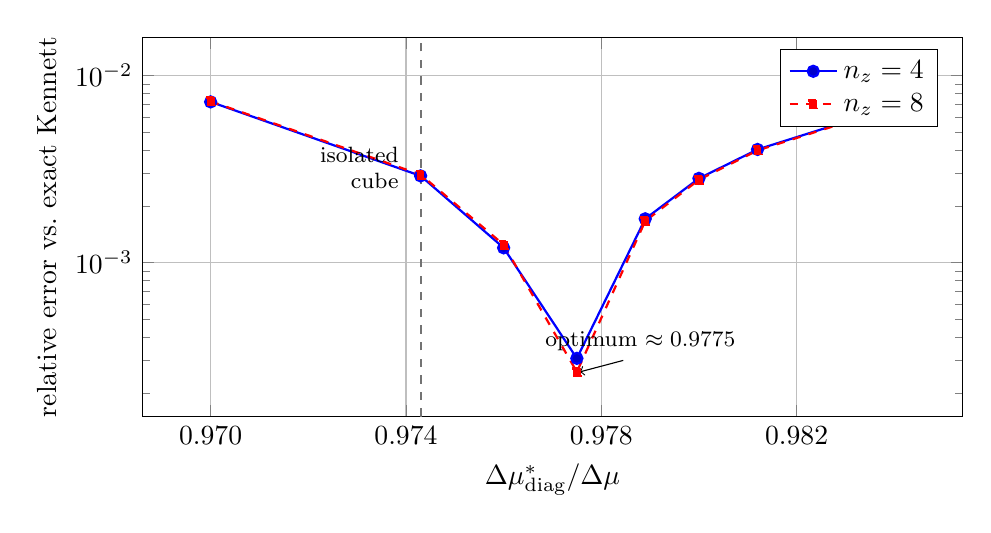
\begin{tikzpicture}
\begin{axis}[
  width=12cm, height=6.4cm,
  xlabel={$\Dmu^*_{\text{diag}}/\Dmu$},
  ylabel={relative error vs.\ exact Kennett},
  ymode=log, grid=major, legend pos=north east,
  every axis plot/.append style={thick},
  xtick={0.970,0.974,0.978,0.982,0.986},
  xticklabel style={/pgf/number format/.cd, fixed, fixed zerofill, precision=3},
  ymin=1.5e-4, ymax=1.6e-2,
]
\addplot coordinates {
 (0.9700,7.22645e-3) (0.9743,2.90671e-3) (0.9760,1.19904e-3) (0.9775,3.07655e-4)
 (0.9789,1.71385e-3) (0.9800,2.81868e-3) (0.9812,4.02391e-3) (0.9840,6.83597e-3)};
\addlegendentry{$n_z=4$}
\addplot[red,dashed,mark=square*,mark size=1.4pt] coordinates {
 (0.9700,7.27333e-3) (0.9743,2.95392e-3) (0.9760,1.24639e-3) (0.9775,2.60192e-4)
 (0.9789,1.66628e-3) (0.9800,2.77102e-3) (0.9812,3.97616e-3) (0.9840,6.78800e-3)};
\addlegendentry{$n_z=8$}
\draw[black!55,dashed,thick] (axis cs:0.974315,1.5e-4) -- (axis cs:0.974315,1.6e-2);
\node[font=\footnotesize,anchor=east,black,align=right]
  at (axis cs:0.97405,3.2e-3) {isolated\\cube};
\node[font=\footnotesize,anchor=south,black] at (axis cs:0.9788,3.0e-4)
  {optimum $\approx0.9775$};
\draw[->,black] (axis cs:0.97845,3.0e-4) -- (axis cs:0.97755,2.6e-4);
\end{axis}
\end{tikzpicture}
\end{center}

The residual behaves as a \emph{single wrong scalar}, with a sharp minimum
displaced from the isolated-cube value --- and \textbf{the minimum sits in the
same place at both refinements}, which is what a per-cell renormalisation must
do and what a numerical artifact would not.

%======================================================================
\section{The law}
%======================================================================

\subsection{Statement}

\begin{tcolorbox}[colback=blue!4,colframe=blue!50!black,
  title=Lattice renormalisation of the shear depolarisation]
In a space-filling cubic lattice, a cube's shear depolarisation is a fixed
fraction of its isolated-cube value:
\[
  1-A^{\text{eff}}_{\varepsilon,\text{diag}}
  \;=\; \Kren\,\bigl(1-A^{\text{iso}}_{\varepsilon,\text{diag}}\bigr),
  \qquad
  \Kren = 0.8862 \quad(\text{static, weak-contrast limit}).
\]
The dilatational and density channels require no correction.
\end{tcolorbox}

\subsection{Universality}

$\Kren$ is constant to $0.3\%$ over a sixteen-fold contrast range, and flat in
frequency until $ka$ grows --- the signature of a static effect:

\begin{center}
\begin{tabular}{lrrrrr}
\toprule
$\Dmu/\mu_0$ & $0.011$ & $0.022$ & $0.044$ & $0.089$ & $0.178$ \\
$\Kren$ & $0.8882$ & $0.8876$ & $0.8879$ & $0.8892$ & $0.8922$ \\
\midrule
$\omega$ & $30$ & $60$ & $120$ & $240$ & $480$ \\
$\Kren$ & $0.8875$ & $0.8879$ & $0.8895$ & $0.8958$ & $0.9204$ \\
\bottomrule
\end{tabular}
\end{center}

Both drifts are first order in their small parameter; extrapolating jointly in
$(\Dmu/\mu_0,\,(ka)^2)$ to the origin gives
\[
  \Kren = 0.886234,
  \qquad
  \partial \Kren/\partial(\Dmu/\mu_0) = +0.018,
  \qquad
  \partial \Kren/\partial (ka)^2 = +33.6 .
\]

\subsection{At the optimum the identity is recovered}

\begin{center}
\begin{tabular}{lrrrrr}
\toprule
$\Dmu/\mu_0$ & $0.011$ & $0.022$ & $0.044$ & $0.089$ & $0.178$ \\
\midrule
residual, isolated cube & $7.3\!\times\!10^{-4}$ & $1.5\!\times\!10^{-3}$ &
  $2.9\!\times\!10^{-3}$ & $5.6\!\times\!10^{-3}$ & $1.0\!\times\!10^{-2}$ \\
residual at the optimum & $1.2\!\times\!10^{-8}$ & $3.1\!\times\!10^{-8}$ &
  $5.6\!\times\!10^{-8}$ & $2.4\!\times\!10^{-7}$ & $3.4\!\times\!10^{-6}$ \\
\bottomrule
\end{tabular}
\end{center}

Five orders of magnitude. \emph{The entire residual is this one scalar.}

\subsection{$8/9$ is excluded}

$8/9=0.888889$ is temptingly close to the raw measurements. The extrapolated
static limit is $0.886234$, below it by $2.65\times10^{-3}$ --- far outside the
scatter of the fit, whose individual points are reproducible to $\sim\!10^{-4}$.
The conjecture is \textbf{refuted}.

The limit lies within $10^{-5}$ of $\sqrt{\pi}/2=0.886227$. This is recorded and
\emph{discounted}: $\sqrt{\pi}/2$ has no evident place in a cubic-lattice
elasticity problem, and $\sqrt{\pi}/d$ is the Ewald splitting parameter used by
the implementation, which makes the coincidence a reason for suspicion rather
than for confidence.

%======================================================================
\section{The corrected solution}
%======================================================================

\subsection{The rule, and the tests that earn it}

Apply $\Kren$ to the shear depolarisation and change nothing else:
$A_{\varepsilon,\text{diag}} \mapsto 1-\Kren\,(1-A_{\varepsilon,\text{diag}})$,
leaving $A_u$, $A_\theta$ and $A_{\varepsilon,\text{off}}$ at their isolated
values. Taken from pure \emph{positive} shear in the static limit, and applied
unchanged:

\begin{center}
\begin{tabular}{lrrr}
\toprule
case & isolated & renormalised & gain \\
\midrule
working (mixed) & $8.51\times10^{-4}$ & $2.22\times10^{-5}$ & $38.3\times$ \\
mixed, $3\times$ contrast & $2.16\times10^{-3}$ & $2.08\times10^{-4}$ & $10.4\times$ \\
pure $\lambda$ (no correction due) & $1.19\times10^{-5}$ & $1.19\times10^{-5}$ & $1.0\times$ \\
pure density (no correction due) & $1.41\times10^{-5}$ & $1.41\times10^{-5}$ & $1.0\times$ \\
\textbf{negative} shear & $3.14\times10^{-3}$ & $7.07\times10^{-5}$ & $44.4\times$ \\
negative mixed & $1.03\times10^{-3}$ & $5.13\times10^{-5}$ & $20.1\times$ \\
\bottomrule
\end{tabular}
\end{center}

Three features make this a prediction rather than a fit:
\begin{enumerate}[nosep]
  \item the constant was extracted from \emph{positive} shear and transfers to
    \textbf{negative} shear at $44\times$;
  \item it leaves the two channels that need no correction \emph{exactly}
    unchanged --- doing nothing where nothing is due is as much a test as
    improving what is;
  \item it was extracted at one contrast and transfers across mixed cases and a
    threefold stronger contrast.
\end{enumerate}

\subsection{Convergence is restored}

This is the structural result, more important than the smaller constant:

\begin{center}
\begin{tabular}{rrrrr}
\toprule
$n_z$ & isolated & ratio & renormalised & ratio \\
\midrule
1 & $7.73\times10^{-4}$ & --- & $1.15\times10^{-4}$ & --- \\
2 & $8.35\times10^{-4}$ & $1.08$ & $4.18\times10^{-5}$ & $0.36$ \\
4 & $8.51\times10^{-4}$ & $1.02$ & $2.22\times10^{-5}$ & $0.53$ \\
8 & $8.58\times10^{-4}$ & $1.01$ & $1.52\times10^{-5}$ & $0.69$ \\
\bottomrule
\end{tabular}
\end{center}

The isolated column saturates at ratio $1.00$; the renormalised one keeps
falling. The discretisation is convergent.

%======================================================================
\section{Status, and what remains}
%======================================================================

\begin{tcolorbox}[colback=orange!6,colframe=orange!55!black,
  title={$\Kren$ is measured, not derived}]
$\Kren$ is universal across contrast and frequency, predictive on cases it was
not fitted to, and reduces the discrepancy by five orders of magnitude at its
optimum. It is nevertheless \textbf{an empirical constant}. No derivation is
offered here, and until one exists $\Kren$ should not be presented as
established physics. It is deliberately \emph{not} wired into the library: the
measurement scripts apply it explicitly so that no result silently depends on an
unproven number.
\end{tcolorbox}

The natural route to a derivation is the difference between the isolated cube's
Eshelby shear component and its space-filling-lattice counterpart --- the same
class of correction as the packing-fraction renormalisation already established
for spheres in this project. Two constraints any derivation must satisfy:
\begin{enumerate}[nosep]
  \item it must produce $0.8862$ and not $8/9$;
  \item it must act on the deviatoric response \emph{only}, leaving the
    dilatational and density channels untouched --- the channel split of \S4.1 is
    a sharp constraint and not every mechanism will respect it.
\end{enumerate}

\paragraph{Reproduction.} Every number in this document is produced by scripts in
the repository, run under the project's environment:

\begin{itemize}[nosep,leftmargin=1.4em]
  \item \S4--\S6, the law and its validation: \\
    \texttt{measure\_shear\_renormalisation.py}
  \item \S2, the prerequisites: \\
    \texttt{gate\_lateral\_sum\_invariance.py},
    \texttt{measure\_representation\_convergence.py}
  \item \S3, the refutations: \\
    \texttt{measure\_residual\_origin.py},
    \texttt{measure\_lattice\_depolarisation.py}
  \item the exact lattice sum underpinning all of it: \\
    \texttt{gate\_lattice\_kupradze.py},
    \texttt{gate\_lattice\_origin.py},
    \texttt{gate\_ewald\_kernel\_wiring.py}
\end{itemize}

\end{document}
